% !TEX encoding = UTF-8 Unicode
% program VLNA -- prida ~ tam kde je pot≈ôeba je soucasti texlive baliku

\pdfoutput=1
\documentclass[twoside,12pt]{article}
% \usepackage[utf8]{inputenc} 
\usepackage[utf8x]{inputenc}
\usepackage[czech]{babel}
\usepackage{dipp}
\usepackage{listings}
\usepackage{pgfplots, pgfplotstable}
\usepackage{filecontents}
\usepackage{comment}
\usepackage{listings}
\usepackage[export]{adjustbox}
\usepackage{float}
\usepackage{caption}

%
%
% START
\begin{document}

\def\,{\penalty10000\hskip.25em}
\pagestyle{headings}
\cislovat{2}

\bakalarska


\titul{Hra založená na rozšířené realitě pro platformu iOS}{Aleš Kocur}{Ing. David Procházka, Ph.D.}{Brno~2015}


\podekovani{
Rád bych poděkoval.. 
}

\prohlasenimuz{V~Brně dne \today}
 
\newpage\null\thispagestyle{empty}\newpage

\abstrakt{
Tato práce se zabývá rozšířenou realitou a jejím využitím ve hrách na~platformě iOS. Zkoumá aktuální přístupy her, které rozšířenou realitu využívají. Práce se zabývá jejich koncepty interakce a přidaných hodnot oproti hrám normálním. Dále jsou představeny frameworky nabízející práci s rozšířenou realitou na mobilní platformě iOS a jejich srovnání na základě vhodnosti pro tvorbu hry. Poslední částí práce je návrh vlastní hry a následná implementace s použitím nejlépe ohodnoceného frameworku.
}{}

\abstract{
EN abstract
}{}


\obsah


Ôªø%
% Úvod a cíl práce
%
\kapitola{Úvod a cíl práce}

% 
\sekce{√övod}
Myšlenku rozšířené reality (angl. Augmented reality) nastínil již před více než sto lety americký spisovatel Lyman Frank Baum \cite{baum}, ale až v posledních letech s nástupem mobilních technologií získává na svém potencionálu více než kdy předtím. Mobilní technologie a přenositelná zařízení nám umožňují pomocí senzorů snímat realitu a obohacovat ji o uměle vytvořené prvky. Toho se dá využít v celé škále odvětví jako je zábavní průmysl, medicína, marketing, vzdělávání, navigace, sport a mnoho dalšího. Tato práce se zabývá aplikací rozšířené reality v zábavním průmyslu, konkrétně hrami. 

% 
% Cíl práce
\sekce{Cíl práce}
Cílem práce je prozkoumat možnosti her v rozšířené realitě na mobilní plaformě iOS a vytvořit hru, které bude rozšířené reality využívat jako obohacujícího prvku pro hráče. Prvním a zároveň velmi důležitým krokem je zvolení správného frameworku na základě výše uvedených kritérií. Poté je potřeba důkladně navrhnout herní systém a jak a do jaké míry se bude hra odehrávat v rozšířené realitě. Dalším krokem bude zaopatření grafických podkladů a modelů pro hru a poslední krok spočívá v samotné implementaci.

%
% Rozšířená realita
%

\kapitola{Rozšířená realita}
Rozšířenou realitou (angl. Augmented reality) je označováno zobrazování digitálních objektů (3D modelů, 2D obrazů) v reálném světě. Tohoto efektu lze dosáhnout pomocí tzv. okna, které nám sdružuje reálné prostředí s virtuálním. Může se jednat o jakoukoliv formu displaye od mobilního telefonu, až po sofistikované nástroje, jako jsou speciální brýle (např. Google Glass). Digitálním objektům je možné pomocí různých technik analýzy obrazu specifikovat pozici, natočení a velikost. Metody vizuálního sledování lze rozdělit do třech základních kategorií \cite{klein_visual_tracking}.

\sekce{Metody vizuálního sledování}
\podsekce{Marker tracking}
Jedním z nejjednodušších a také nejspolehlivějších rozpoznávacích technik postavení objektů je Marker Tracking. Jedná se většinou o černobíle čtvercové QR kódy, které uchovávají informaci o svém identifikačním čísle, orámované černým okrajem o pevné velikosti. Na základě přečteného identifikátoru lze přiřazovat jednotlivým markerům různé objekty. Černé rámování slouží k analýze vzdálenosti od markeru, jeho natočení a velikost. Tato metoda je velmi efektivní, analýza takového markeru na zařízení iPhone 5 s frameworkem Metaio v obrazu zabere průměrně 4,3 ms (na základě vlastního měření).

\begin{figure}[H]
    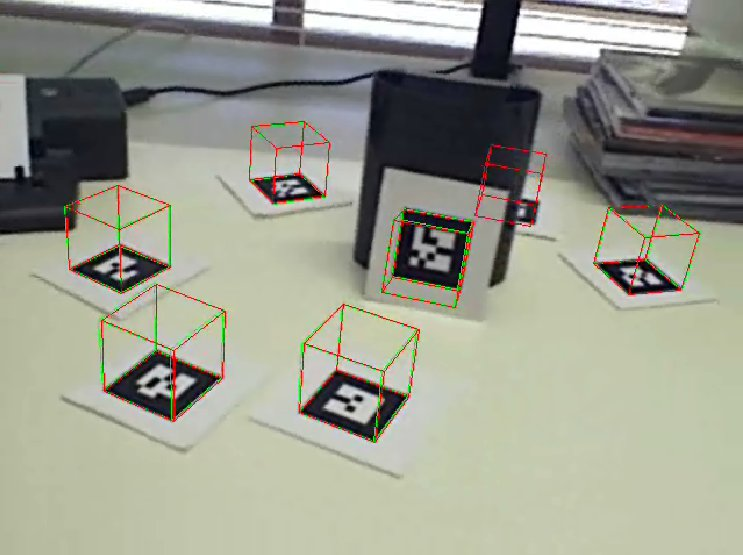
\includegraphics[width=350px, center]{images/marker-tracking.jpg}
    \caption{Marker tracking}
    \label{marker_tracking}
\end{figure}

\podsekce{Markerless tracking}
Další možností jak umisťovat objekty do rozšířené reality je pomocí tzv. Markerless trackingu. Jedná se o princip podobný Marker trackingu s tím rozdílem, že namísto markerů jsou použity libovolné obrazy. Při analýze je pak potřeba vlastnit digitální predlohu takového obrázu a vyhledávat jej ve snímané realitě. Na základě porovnání natočení obrazu ve snímané realitě a předlohy je zjištěna aktuální vzdálenost od objektu, velikost a natočení. Tento princip analýzy je pomalejší oproti Marker trackingu a při nevhodné volbě předlohy (nízký kontrast barev) méně spolehlivý, zvláště při špatných světelných podmínkách.

\begin{figure}[H]
    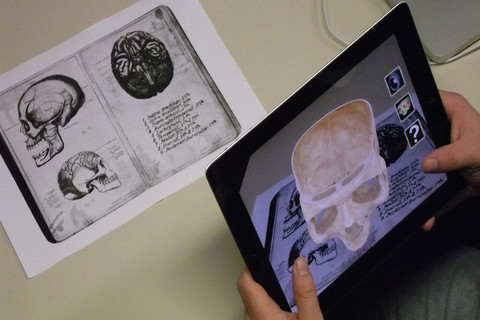
\includegraphics[width=350px, center]{images/markerless-tracking.jpg}
    \caption{Markerless tracking}
    \label{markerless_tracking}
\end{figure}

\podsekce{Sledování neznámých prostředí}
Umisťovat virtuální objekty do snímané reality lze i bez známých vzorů a to pomocí detekce hran na základě pohybu kamery. Nejrozšířenější systémy takovéto analýzy jsou SLAM (Simultaneous localization and mapping) a jeho vylepšení PTAM (Parallel Tracking and Mapping). PTAM je vyvíjen Active Vision Laboratory na University of Oxford a od roku 2014 volně dostupný pod licencí GNU GPLv3. Tento systém dokáže analyzovat plochy a hrany v obrazu a na základě těchto informací pak vykreslovat správně umístěné a natočené virtuální objekty. Tyto systémy mají uplatnění mimo jiné také při navigaci autopilotovaného vozidla, vesmírných vozů a podobně.

\begin{figure}[H]
    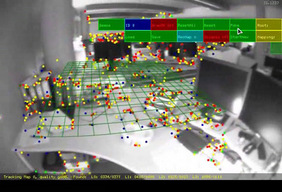
\includegraphics[width=350px, center]{images/slam.jpg}
    \caption{SLAM: Simultaneous localization and mapping}
    \label{slam}
\end{figure}


%
% Aktuální hry a jejich koncepty
%

\kapitola{Využití rozšířené reality, koncepty využité ve hrách}
Rozšířená realita nabývá s vývojem stále výkonější mobilních telefonů na atraktivitě a rozšiřuje se i v komerční svéře. Mobilní aplikace dokáží interagovat s realitou např. přehráváním trailerů k filmům nad jeho plakátem, vizualizovat návrhy staveb nad prospekty nebo vizualizovat učební materiál v interaktivních učebnicích. Využití rozšířené reality je nespočetné a s přibývající dostupností technologií roste i počet nápadů na její uplatnění. Velké oblibě se těší zejména ve hrách, kde využívá prostředí hráče jako herní plochu a mobilní telefon jako okno do rozšířené reality.

\sekce{Interakce se zařízením}
Tento koncept je postaven na principu interakce hráče pouze se zařízením. Hráč vůbec nemanipuluje ani neinteraguje s prvky herního pole. Tento koncept je vhodný pro zejména pro typy her ve kterých nepotřebujeme pohybovat s objekty a je charakteristický pro mapově (geolokačně) založené hry -- objekty jsou umisťovány do reálného světa s koodináty. Typickým představitelem takového konceptu je hra Ingress.

%
% Ingress
% 

\podsekce{Ingress}
Masově multiplayerová online hra vyvíjená startupem Niantics Labs, kterou zaštiťuje Google, dostupná pro iOS i Android. Celá hra má v pozadí příběh o \uv{Exotické hmotě} (Exotic Matter), která byla objevena vědci z CERNu, a je to zárodek mimozemského druhu zvaného Shapers. Osvícení (The Enlightened), jedna ze dvou frakcí, věří, že toto je úsvit nového věku. Druhá frakce, Rezistence (The Resistance) naopak brojí proti těmto mimozemským silám. Hra spočívá ve vytváření frakčních portálů na různých místech, zejména na městských památkách, veřejných budovách a podobně. Hráči chodí s telefony po městě a vytvářením takovýchto portálů přivlastňují danná uzemí své frakci. Mohou také stavět obranné prvky a bránit tak tyto portály před napadením frakce druhé. Zobrazování rozšířené reality je zjednodušené, pouze černé pozadí s obrysy některých budov. Hra se tedy více než na rozšířenou realitu zaměřuje na příběh a rozšířená realita zde slouží pouze jako část celé hry. Více informací lze získat na oficiálních webových stránkách hry www.ingress.com \cite{ingress}.


\begin{figure}[H]
    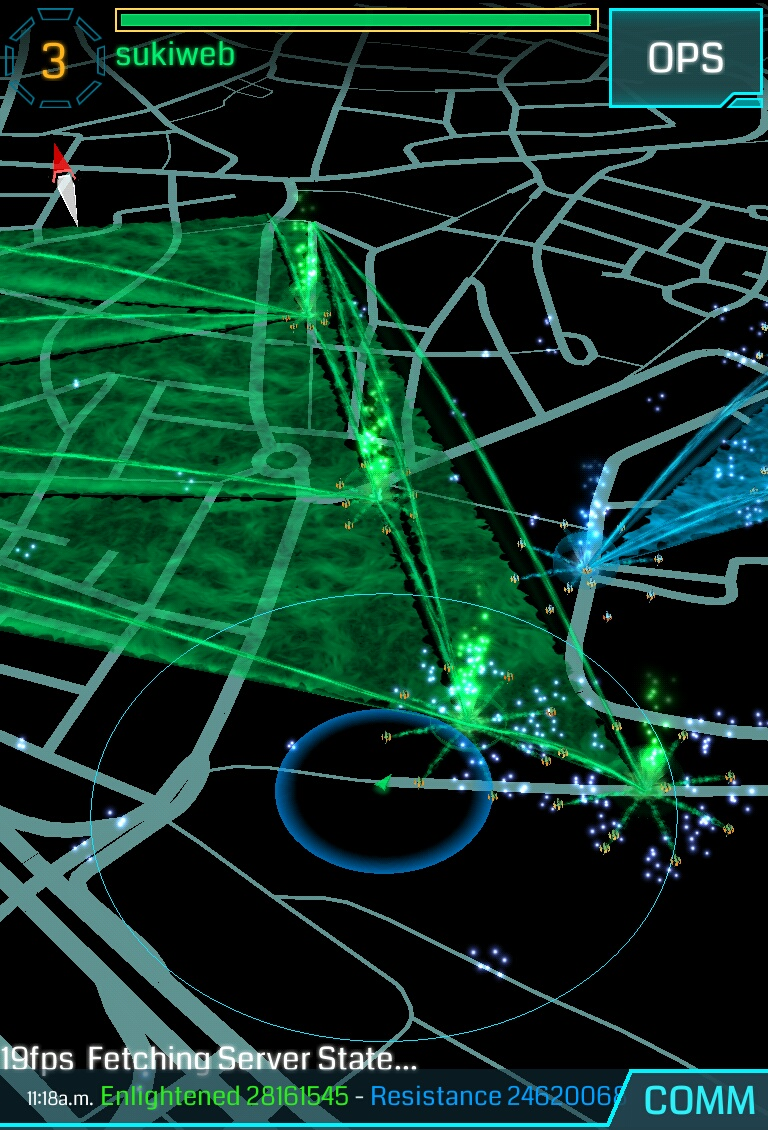
\includegraphics[width=320px, center]{images/ingress.jpg}
    \caption{Screenshot ze hry Ingress}
    \label{ingress_screenshot}
\end{figure}

\sekce{Interakce s herní deskou}
Dalším konceptem je interakce s herní deskou, kdy hráč interaguje pomocí gest nebo stisknutím virtuálních tlačítek na desce. Tento koncept štěpí interakční část a zobrazovací (hráč manipuluje s prvky na desce, ale výsledek vidí pouze přes zařízení) a pro uživatele může být v případech mobilního telefonu obzvlášť nepříjemný na ovládání, více vhodný je například na brýle. Z tohoto důvodu je také tento koncept v mobilních hrách téměř nepoužívaný. Mezi hry využívající tohoto přístupu jsou povětšinou hry původem deskové či karetní a rozšířenou realitu zde využívají spíše pro zvýšení intenzity zážitku ze hry vizualizacema procesů, které si jinak člověk musí pouze představovat. 

%
% Drakerz-Confrontation 
%

\podsekce{Drakerz Confrontation}
Karetní hra vyvíjená od roku 2010 francouzskou firmou Peoleo s první alpha verzí vydanou roku 2013 ve Francii \cite{venturebeat}. Dnes je hra dostupná pouze pro PC a nejsou žádné informace, zda dorazí v budoucnu i na mobilní platformy. Drakerz Confrontation hráči mají karty s různými typy draků s různými vlastnostmi a schopnostmi. Hra využívá rozšířené reality k vizualizaci draků nad kartami položenými na stole. Ke hraní je potřeba vlastnit kameru připojitelnou k PC, na kterém se pak vizualizace zobrazují. Vizualizované jsou jak pohyby draků po herní ploše, tak např. boje i prostoje. Více informací lze nalézt na oficiálních stránkách hry www.drakerz.com \cite{peoleo_about}, kde je také možné zakoupit karty nebo hru stáhnout.


\begin{figure}[H]
    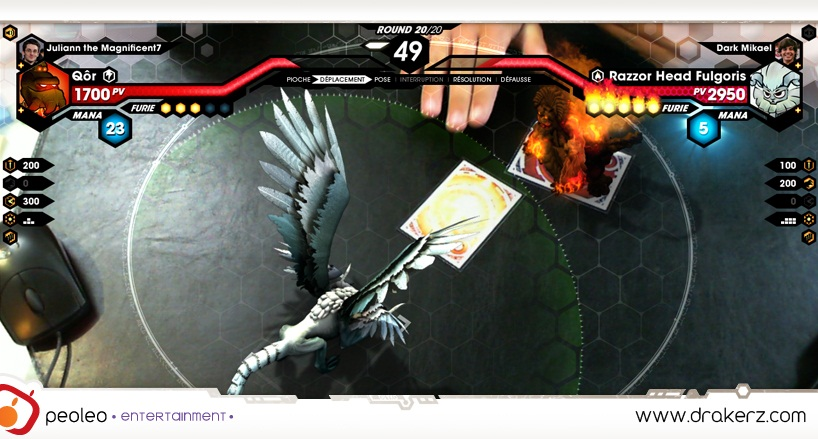
\includegraphics[width=424px, center]{images/drakerz-confrontation.jpg}
    \caption{Screenshot ze hry Drakerz Confrontation}
    \label{drakerz_screenshot}
\end{figure}

\sekce{Smíšená interakce}
Tento koncept kombinuje předchozí dva uvedené. Hráč v tomto případě primárně používá zařízení, ale má i možnost ovládat herní prvky v reálném prostřední na herní desce. Typickým příkladem smíšené interakce je hra ARHrrrr!.

% 
% ARHrrrr!
\podsekce{ARHrrrr!}
Jednou z populárních her je hra ARhrrrr! z dílny Georgia Tech Augmented Environments Lab, která využívá vytištěné hrací plochy k vizualizaci části města (Markerless tracking), kterou napadají zombie a hráč v roli snipera v helikoptéře se pohybuje nad hrací plochou a střílí. Tento koncept herní plochy kombinované s interakcí pomocí mobilního zařízení využívá většina her a to z důvodu zachování veškeré uživatelské interakce na jednom místě, na zařízení. Hra je obohacena o různé doplňky, například položením bonbónu Skittles na herní plochu vznikne nášlapná mina, kterou můžeme kliknutím na ni odjistit (příklad interakce s herní plochou). Různé barvy bonbónů mají navíc různé funkce.

\begin{figure}[H]
    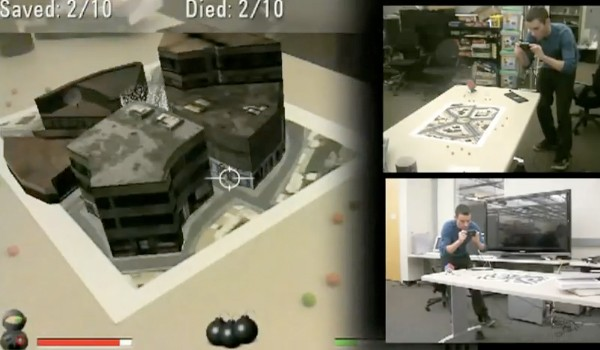
\includegraphics[width=424px, center]{images/arhrrrr.jpg}
    \caption{Screenshot ze hry ARhrrrr!}
    \label{arhrrrr_screenshot}
\end{figure}


% 
% Nova stranka
\newpage 

\kapitola{Framework}

\sekce{Kritéria hodnocení}
Kritéria hodnocení se odvíjí od náročnosti požadavků na aplikaci, v tomto případě hra. Je tedy důležité, aby framework uměl dobře pracovat s 3D modely a provádět animace, aby hra byla zajímavá. Dalším aspektem je rychlost závislá na počtu zobrazovaných objektů a posledním neméně důležitým faktorem jsou licenční podmínky pro používání.

\sekce{Přehled frameworků}

\podsekce{ARToolKit}
ARToolkit byl původně vyvinut Hirokazu Katou na Nara Institute of Science and Technology v roce 1999. Nyní je udržován The Human Interface Technology Lab na University of Washington jako open source projekt s komerčníma licencema od ARToolWork. Tento framework je dostupný pro všechny majoritní platformy (Windows, Linux, Mac OS X, SGI) s různými porty pro mobilní operační systémy (iOS, Android). Mobilní verze tohoto frameworku portují již konkrétní firmy a vydávají jako vlastní produkt, nejsou tedy volně dostupné –- nepodařilo se sestavit testovací projekt pro tento framework a benchmarky uvedené v dokumentaci jsou velmi nepřesně specifikované (chybí specifikace hardwaru, na kterém byly tyto měření prováděny). 

\begin{figure}[H]
    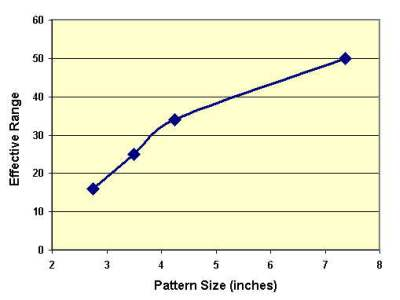
\includegraphics[width=324px, center]{images/artoolkit_benchmark.jpg}
    \caption{Chyba sledování závislá na velikosti markeru}
    \label{artoolkit_benchmark}
\end{figure}

Mezi hlavní fukce frameworku patří kamerově pozicované a orientováné sledování, sledování černých čtverců s možností definice vlastních typů, jednoduchá kalibrace kamer \cite{artoolkit_features}. Podpora vykreslování modelů je pouze nízkoúrovňová, lze renderovat objekty pomocí OpenGL. Většinou je využit v projektech jako část komplexního toolkitu pro práci s rozšířenou realitou např. OSGART (kombinace ARToolKit a OpenSceneGraph) \cite{osgart} nebo ARToolKitPlus (rozšířená verze ARToolKitu, vývoj ukončen roku 2006) \cite{wagner_schmalstieg}. 

\podsekce{Metaio}
Metaio je multiplatformní framework který vyvíjí stejnojmenná německá firma od roku 2003. Mezi produkty Metaio najdeme framework pro rozšířenou realitu na všechny majoritní platformy a také sadu aplikačních nástrojů specializující se na usnadnění práce i samotný vývoj bez programování. Metaio pro iOS je dostupné jako C++ framework. 
Dokumentace uvádí měření, ukazující udržení výkonu vykreslování 60 snímků za vteřinu (FPS) při 200 000 polygonech na iPhone 5S.

\begin{figure}[H]
\centering
    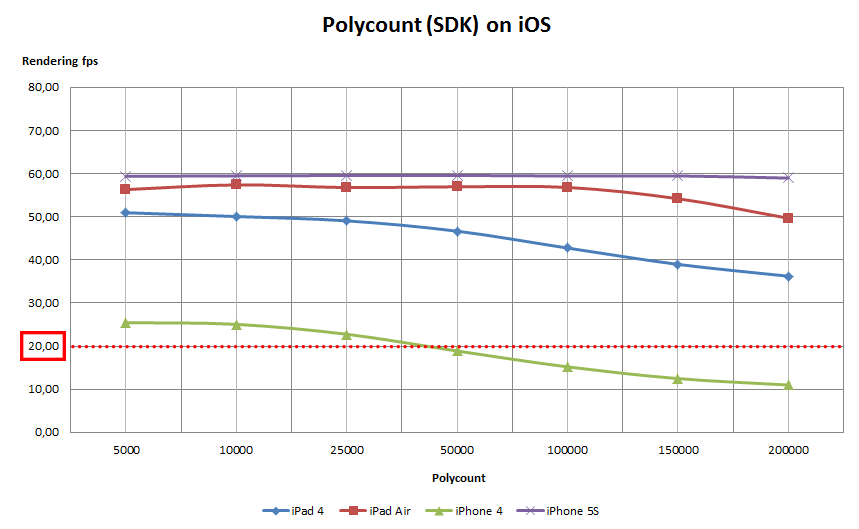
\includegraphics[width=424px, center]{images/Polycount_SDK_iOS_20fps.png}
\captionsetup{justification=centering}
    \caption{Rychlost vykreslování (v FPS) pro jednotlivé iOS zařízení závislé na počtu vykreslovaných polygonů}
    \label{metaio_benchmark}
\end{figure}

Také byl vytvořen testovací projekt, jehož jedinýmúkolem bylo rozeznávat 20 různých markerů. Na tomto projektu pak byly provedeny zkoušky rychlosti nalezení markeru v obrazu. Test byl prováděn na zařízení iPhone 5 (model A1429) firmy Apple. Z výsledných hodnot byl vypočítán průměr 4,31 ms. 


Metaio SDK dokáže pracovat s modely ve formátech OBJ, MD2 a FBX a podporuje také jejich animace. Pod podmínkou vodoznaku a nemožnosti publikovat aplikaci na AppStore nabízí volnou licenci na všechny verze svého frameworku. 

\podsekce{Qualcomm Vuforia}
Jedná se o poměrně nový framework vyvíjený od roku 2011 a nabízí velké množství funkcí. Jako hlavní lze uvést tzv. markerless recognition (možnost vykreslovat objekty nad obrázky), podporu frameworku Unity (framework usnadňující vývoj 3D her) nebo takzvané virtuální tlačítka (Virtual buttons, tlačítka promítaná do virtuální reality a interakce s nimi). Samotný framework nabízí aplikační rozhraní pro C++, Javu, Objective-C a .NET, což významným způsobem usnadňuje portace aplikace na různé platformy. Široké spektrum funkcí se odráží na licenčních podmínkách frameworku, u neplacených licencí je omezen počet rozpoznaných objektů (pozn. v průběhu tvorby této práce byly změněny licenční podmínky a framework je dostupný zdarma s vodoznakem a nemožností publikovat aplikaci). Velkým mínusem je stejně jako v případě ARToolKitu pouze nízkoúrovňová podpora vykreslování objektů pomocí OpenGL. Pro podporu zobrazování modelů ve formátech např. OBJ, FBX a podobně je potřeba využít nějaké další pomocné knihovny \cite{vuforia_3dformats}.

\podsekce{Augmented kit}
Framework psaný čistě pro platformu iOS a tedy v Objective-C. Vyniká jednoduchým API a dobrou dokumentací. Nabízí pouze základní služby vykreslovaní objektů na markerech, či GPS souřadnic a gyroskopu. Framework je vyvíjen teprve od roku 2012 firmou Luteg Software Technologies a to se projevuje velmi malou vývojářskou základnou. Na druhou stranu má přívětivé licenční podmínky, kdy poskytuje volnou licenci pod podmínkou vodoznaku a nemožnosti aplikaci publikovat na AppStore. 

\sekce{V√Ωbƒõr frameworku}

% 
% Nova stranka
\newpage
\kapitola{Metaio}
\sekce{Formát 3D modelů}
Základem dobrého návrhu aplikace je správná volba technologií. Mezi ně v tomto případě patří i volba formátu pro 3D modely. Framework Metaio podporuje renderování objektů ve formátech OBJ, MD2 a FBX. Pro tvorbu modelů byl použit 3D modelovací nástroj 3Ds Max od firmy Autodesk a to čistě z důvodů základní znalosti tohoto softwaru. Tato práce se nezabývá porovnáváním modelovacích softwarů. Kritérii pro výběr formátu jsou podpora exportu z 3Ds Max, podpora animací, podpora textur.

\podsekce{OBJ}
Otevřený formát vyvinutý firmou Wavefront Technologies pro přenos 3D objektů. Formát specifikuje pozice každého vertexu v objektu, UV souřadnice textury vertexu a plochy (faces) každého polygonu \cite{obj_wiki}. Obsahuje podporu textur pomocí přiložených materiálů ve formátu MTL (Material Template Library). Formát OBJ je standardně textový formát, může se však vyskytovat i v binární podobě. Takovýto binární soubor má pak příponu .mod. Formát bohužel nemá podporu animací \cite{obj_doc} a tím nevyhovuje v jednom ze tří bodů daných kritérií.

\podsekce{MD2}
Formát MD2 se stal populárním díky firmě id Software's \cite{md2_wiki}, která jej použila v id Tech 2 známý jako Quake II engine \cite{quake_engine} pro modely všech postav ve hře Quake II a dalších, rovněž postavených na tomto enginu. MD2 má podporu key-frame animací a textur. MD2 byl později nahrazen novějším formátem MD3 \cite{id_tech_3_wiki}. Tento formát je nyní již zastaralý a nemá valnou podporu v 3Ds Maxu, vyjma komerčního pluginu \cite{qtip_plugin}. 

\podsekce{FBX}
Proprietární formát FBX (FilmBoX) je od roku 2006 vyvíjen a spravován firmou Autodesk \cite{autodesk_fbx}. Firma pro užívání tohoto formátu vydala FBX SDK, který umožňuje zapis, čtení a konverze tohoto formátu \cite{autodesk_fbx_sdk}. Formát podporuje animace, textury a jelikož je vyvíjen stejnou firmou jako 3Ds Max, má v tomto softwaru i náležitou podporu pro export.


\begin{table}[H]
\centering
\begin{tabular}{|c|c|c|c|}
\hline
Formát & Podpora animací & Podpora textur & Podpora exportu 3Ds Max  \\ \hline
OBJ    & Ne              & Ano            & Ano                      \\ \hline
MD2    & Ano             & Ano            & Pouze komerčním pluginem \\ \hline
FBX    & Ano             & Ano            & Ano                      \\ \hline
\end{tabular}
\caption{Shrnutí kritérií pro formáty}
\end{table}


Na základě daných kritérií byl zvolen za nejvhodnější formát FBX. Metaio sice podporuje tento formát, ale využívá k tomu utility zvané MeshConvertor, které je potřeba dodat FBX model s případnými UV mapami textur modelu. Výsledným souborem je archiv formátu ZIP, který obsahuje informace o daném modelu, přiložené textury, názvy animací a metadata. Tento zip lze pak již lze snadno používat v Metaio SDK.


% 
% Nova stranka
\newpage

\kapitola{ARCity}

% 
% Nova stranka
\newpage

%
% Z√°vƒõr
%
\kapitola{Z√°vƒõr}
Z√°vƒõr

%
% Návrhy na vylepšení
\sekce{Návrhy na vylepšení}

%
%
% Přílohy
\kapitola{Přílohy}
Na přiloženém CD jsou k dispozici tyto přílohy: 
\begin{itemize}
\item priloha1
\end{itemize}


% 
% Literatura
% 
\begin{literatura}

\citace{baum}{BAUM, 1901} {
	\autor{L. Frank Baum}
	\nazev{The Master Key: An Electrical Fairy Tale, Founded Upon the Mysteries of Electricity and the Optimism of Its Devotees}
	BiblioBazaar, 2006, ISBN 978-1426409240
}


\citace{klein_visual_tracking}{Klein, 2012}
{
	\autor{KLEIN, Georg.}
	\nazev{Visual Tracking Methods for Augmented Reality. }
	 [online]. [cit. 2015-03-31]. Dostupné z: 		http://www.raeng.org.uk/publications/other/georg-klein-presentation-frontiers-of-engineering
}

\citace{peoleo_about}{Peoleo, 2015}
{
	\autor{Peoleo}
	\nazev{Drakerz-Confrontation About}
	 [online]. [cit. 2015-03-31]. Dostupné z: http://www.drakerz.com/qu-est-ce-que-drakerz.html/
}

\citace{venturebeat}{Venture Beat, 2014}
{
	\autor{Venture Beat}
	\nazev{Drakerz-Confrontation augmented-reality card game launches in the U.S.}
	 [online]. [cit. 2015-03-31]. Dostupné z: http://venturebeat.com/2014/07/01/drazkerz-confrontation-augmented-reality-card-game-launches-in-the-u-s/
}

\citace{ingress}{Niatics Labs, 2015}
{
	\autor{Niatics Labs}
	\nazev{Ingress official website}
	 [online]. [cit. 2015-04-01]. Dostupné z: https://www.ingress.com/
}

\citace{obj_wiki}{Wikipedia, 2015}
{
	\autor{Wikipedia}
	\nazev{Wikipedia}
	 [online]. [cit. 2015-04-02]. Dostupné z: http://en.wikipedia.org/wiki/Wavefront\_.obj\_file
}

\citace{obj_doc}{Paul Burke, 2015}
{
	\autor{Paul Burke}
	\nazev{Object Files (.obj)}
	 [online]. [cit. 2015-04-02]. Dostupné z: http://paulbourke.net/dataformats/obj/
}

\citace{quake_engine}{M.H. Williams, 2011}
{
	\autor{M.H. Williams}
	\nazev{id Software Wants To Shorten Dev Cycles}
	 [online]. [cit. 2015-04-02]. Dostupné z: http://web.archive.org/web/20110827005123/http://www.industrygamers.com/news/id-software-wants-to-shorten-dev-cycles/
}

\citace{md2_wiki}{Wikipedia, 2015}
{
	\autor{Wikipedia}
	\nazev{Wikipedia}
	 [online]. [cit. 2015-04-02]. Dostupné z: http://en.wikipedia.org/wiki/MD2\_\%28file\_format\%29
}

\citace{id_tech_3_wiki}{Wikipedia, 2015}
{
	\autor{Wikipedia}
	\nazev{Wikipedia}
	 [online]. [cit. 2015-04-02]. Dostupné z: http://en.wikipedia.org/wiki/Id\_Tech\_3
}

\citace{qtip_plugin}{QTiP, 2015}
{
	\autor{QTiP}
	\nazev{QTiP}
	 [online]. [cit. 2015-04-02]. Dostupné z: http://www.qtipplugin.com/
}

\citace{autodesk_fbx}{Autodesk, 2015}
{
	\autor{Autodesk}
	\nazev{FBX}
	 [online]. [cit. 2015-04-02]. Dostupné z: http://www.autodesk.com/products/fbx/overview
}

\citace{autodesk_fbx_sdk}{Autodesk, 2015}
{
	\autor{Autodesk}
	\nazev{FBX SDK}
	 [online]. [cit. 2015-04-02]. Dostupné z: http://usa.autodesk.com/adsk/servlet/pc/item?siteID=123112\&id=10775847
}

\citace{artoolkit_features}{HITLab, 2015}
{
	\autor{The Human Interface Technology Lab, University of Washington}
	\nazev{Feature list}
	 [online]. [cit. 2015-04-02]. Dostupné z: http://www.hitl.washington.edu/artoolkit/documentation/features.htm
}

\citace{osgart}{HITLab NZ, 2015}
{
	\autor{The Human Interface Technology Laboratory New Zealand}
	\nazev{OSGART website}
	 [online]. [cit. 2015-04-02]. Dostupné z: https://www.artoolworks.com/community/osgart/
}

\citace{wagner_schmalstieg}{WAGNER, SCHMALSTIEG, 2007}
{
	\autor{Daniel Wagner and Dieter Schmalstieg}
	\nazev{ARToolKitPlus for Pose Tracking on Mobile Devices}
In Proc. 12th Computer Vision Winter Workshop (CVWW'07), Sankt Lambrecht, Austria, February 2007
}

\citace{vuforia_3dformats}{Qualcomm, 2015}
{
	\autor{Qualcomm}
	\nazev{3D File Formats}
	 [online]. [cit. 2015-04-02]. Dostupné z: https://developer.vuforia.com/library/articles/Solution/3D-File-Formats
}




% Obrazky

\citace{ingress_screenshot}{Flickr, 2015}
{
	\autor{Yahoo Inc.}
	\nazev{Flickr}
	[online]. [cit. 2015-04-02]. Flickr
	Obrázek ve formátu: JPEG. Dostupné z: https://farm9.staticflickr.com/8219/8266348091\_08fe415355\_o.jpg
}

\citace{drakerz_screenshot}{Game guide, 2015}
{
	\autor{Game guide}
	\nazev{Game guide}
	[online]. [cit. 2015-04-02]. Game guide
	Obrázek ve formátu: JPEG. Dostupné z: http://game-guide.fr/wp-content/uploads/2014/03/drakerz-confrontation-05.jpg
}

\citace{arhrrrr_screenshot}{Engadget, 2015}
{
	\autor{Engadget}
	\nazev{Engadget}
	[online]. [cit. 2015-04-02]. Engadget
	Obrázek ve formátu: JPEG. Dostupné z: http://www.blogcdn.com/www.engadget.com/media/2009/06/arhrrrr-pic-rm-eng.jpg
}

\citace{marker_tracking}{VTTResearch, 2015}
{
	\autor{VTTResearch}
	\nazev{Marker tracking}
	[online]. [cit. 2015-04-02]. VTTResearch
	Obrázek ve formátu: JPEG. Dostupné z: http://virtual.vtt.fi/virtual/proj2/multimedia/media/images/MultiMarker.jpg
}

\citace{markerless_tracking}{Wikipedia, 2015}
{
	\autor{Wikipedia}
	\nazev{Wikipedia}
	[online]. [cit. 2015-04-02]. Wikipedia.org
	Obrázek ve formátu: JPEG. Dostupné z: http://upload.wikimedia.org/wikipedia/commons/f/f4/App\_iSkull,\_an\_augmented\_human\_skull.jpg
}

\citace{slam}{Department of Engineering Science, University of Oxford, 2008}
{
	\autor{Department of Engineering Science, University of Oxford}
	\nazev{SLAM}
	[online]. [cit. 2015-04-02]. 
	Obrázek ve formátu: JPEG. Dostupné z: http://www.robots.ox.ac.uk/~lav/Papers/castle\_etal\_iswc2008/castle\_etal\_iswc2008.jpg
}

\citace{artoolkit_benchmark}{HITLab, 2015}
{
	\autor{The Human Interface Technology Lab, University of Washington}
	\nazev{ARToolKit Benchmarks}
	[online]. [cit. 2015-04-03]. 
	Obrázek ve formátu: JPEG. Dostupné z: http://www.hitl.washington.edu/artoolkit/documentation/benchmark.htm
}

\citace{metaio_benchmark}{Metaio, 2015}
{
	\autor{Metaio GmbH}
	\nazev{Metaio iOS polycount}
	[online]. [cit. 2015-04-03]. 
	Obrázek ve formátu: JPEG. Dostupné z: http://dev.metaio.com/sdk/documentation/content-creation/3d-animation/polygon-count/general-guidelines/
}





%
%\citace{template}{Venture Beat, 2014}
%{
%	\autor{Venture Beat}
%	\nazev{Drakerz-Confrontation augmented-reality card game launches in the U.S.}
%	 [online]. [cit. 2015-03-31]. Dostupné z: http://venturebeat.com/2014/07/01/drazkerz-confrontation-augmented-reality-card-game-launches-in-the-u-s/
%}




\end{literatura}


\end{document}
